%% Patent Application: Resonance Fingerprinting Methods for Protein Quality
%% Control and Diagnostics
%% Inventor: Jonathan Washburn
%% Contact: washburn.jonathan@gmail.com
%% Filing Date: January 2026

\documentclass[12pt,letterpaper]{article}

\usepackage[margin=1in]{geometry}
\usepackage{amsmath,amssymb,amsfonts}
\usepackage{graphicx}
\usepackage{tikz}
\usetikzlibrary{shapes,arrows,positioning,calc,patterns}
\usepackage{booktabs}
\usepackage{array}
\usepackage{enumitem}
\usepackage{fancyhdr}
\usepackage{xcolor}
\usepackage{hyperref}
\usepackage{setspace}

% Patent-style formatting
\setlength{\parindent}{0.5in}
\setlength{\parskip}{0.5em}
\onehalfspacing

% Header
\pagestyle{fancy}
\fancyhf{}
\rhead{Patent Application}
\lhead{Washburn}
\rfoot{Page \thepage}

\hypersetup{
    colorlinks=true,
    linkcolor=blue,
    urlcolor=blue,
    citecolor=blue
}

% Custom colors
\definecolor{pass}{RGB}{50,180,50}
\definecolor{fail}{RGB}{200,50,50}
\definecolor{warning}{RGB}{200,150,50}
\definecolor{fingerprint}{RGB}{100,100,200}

\begin{document}

%% ============================================================================
%%                              TITLE PAGE
%% ============================================================================

\begin{center}
\vspace*{0.8in}

{\LARGE \textbf{PATENT APPLICATION}}

\vspace{0.4in}

{\Large \textbf{RESONANCE FINGERPRINTING METHODS}}

{\Large \textbf{FOR PROTEIN QUALITY CONTROL}}

{\Large \textbf{AND DIAGNOSTICS}}

\vspace{0.8in}

\textbf{PROVISIONAL PATENT APPLICATION}

\vspace{0.5in}

\begin{tabular}{ll}
\textbf{Inventor:} & Jonathan Washburn \\
\textbf{Email:} & washburn.jonathan@gmail.com \\
\textbf{Filing Date:} & January 17, 2026 \\
\textbf{Application Type:} & Utility Patent (Provisional) \\
\textbf{Related Applications:} & Patents 001--006 \\
\end{tabular}

\vspace{0.8in}

\textit{Methods for characterizing proteins using resonance frequency fingerprinting, including frequency sweep protocols, resonance curve fitting, extraction of fingerprint metrics, classification of proteins and variants, prediction of aggregation propensity, qualification of manufacturing lots, and isotope-shift verification for mechanism confirmation.}

\vfill

\textbf{CONFIDENTIAL --- PATENT PENDING}

\end{center}

\newpage

%% ============================================================================
%%                         TABLE OF CONTENTS
%% ============================================================================

\tableofcontents
\newpage

%% ============================================================================
%%                              ABSTRACT
%% ============================================================================

\section*{ABSTRACT OF THE DISCLOSURE}
\addcontentsline{toc}{section}{ABSTRACT OF THE DISCLOSURE}

Methods for characterizing proteins and assessing quality using resonance fingerprinting based on the molecular gate frequency. The methods comprise: (a) performing a frequency sweep across the molecular gate frequency range (12--17 GHz for H$_2$O, 8--13 GHz for D$_2$O) while monitoring protein folding response; (b) fitting the resulting resonance curve to extract fingerprint metrics including center frequency, resonance width, resonance depth, and asymmetry; (c) using these metrics to classify proteins, identify variants, predict aggregation propensity, and qualify manufacturing lots; (d) confirming the resonant mechanism by verifying a $\sqrt{2}$ isotope shift in D$_2$O; and (e) generating pass/fail or graded quality assessments based on comparison to reference fingerprints. The methods enable non-destructive, rapid ($<$ 10 minutes), label-free characterization of protein folding properties with applications in biopharmaceutical manufacturing quality control, lot release testing, stability assessment, biosimilar comparison, and research protein characterization. The fingerprint metrics are derived from the Recognition Science framework and the molecular gate timescale $\tau_{19} \approx 68$ ps. Machine-verified proofs ensure the predicted frequency ranges are mathematically correct.

\vspace{1em}
\noindent\textbf{Keywords:} protein fingerprinting, quality control, resonance curve, aggregation prediction, lot qualification, biosimilar, frequency sweep, molecular gate, isotope verification

\newpage

%% ============================================================================
%%                      BACKGROUND OF THE INVENTION
%% ============================================================================

\section{BACKGROUND OF THE INVENTION}

\subsection{Field of the Invention}

The present invention relates generally to methods for protein characterization and quality control, and more specifically to resonance fingerprinting methods using the molecular gate frequency for assessing protein folding properties, classifying proteins, predicting aggregation, and qualifying manufacturing lots.

\subsection{Description of Related Art}

\subsubsection{Current Protein Quality Control Methods}

Biopharmaceutical manufacturers use various methods to characterize protein products:

\begin{table}[h]
\centering
\begin{tabular}{llll}
\toprule
\textbf{Method} & \textbf{Property} & \textbf{Time} & \textbf{Limitations} \\
\midrule
SDS-PAGE & Size, purity & 2--4 hours & Destructive, qualitative \\
SEC-HPLC & Aggregates & 30--60 min & Limited to soluble aggregates \\
Mass spectrometry & Sequence, modifications & Hours & Complex, expensive \\
Circular dichroism & Secondary structure & 15--30 min & Low sensitivity \\
DSC & Thermal stability & 1--2 hours & Destructive \\
DLS & Particle size & 5--15 min & Limited structural info \\
FTIR & Secondary structure & 10--30 min & Sample prep required \\
\bottomrule
\end{tabular}
\caption{Current protein characterization methods}
\end{table}

\subsubsection{Limitations of Prior Art}

\begin{enumerate}[label=(\alph*)]
\item \textbf{No folding dynamics assessment:} Current methods assess static structure or aggregate state, not the dynamic folding properties that determine stability and function.

\item \textbf{Slow turnaround:} Many methods require hours, limiting throughput in manufacturing settings.

\item \textbf{Destructive testing:} Many methods consume or alter the sample, preventing further use.

\item \textbf{Label requirements:} Some sensitive methods require fluorescent labels or other modifications.

\item \textbf{No predictive power:} Current methods detect existing problems but do not predict future aggregation or stability issues.

\item \textbf{No mechanistic information:} Methods measure symptoms (aggregates, structure) but not underlying folding dynamics.
\end{enumerate}

\subsubsection{The Need for Folding Dynamics Assessment}

What is needed is a characterization method that:

\begin{enumerate}[label=(\arabic*)]
\item Assesses \textbf{folding dynamics}, not just static structure;
\item Is \textbf{rapid} ($<$ 10 minutes per sample);
\item Is \textbf{non-destructive} and label-free;
\item Provides \textbf{predictive} information about stability and aggregation;
\item Generates \textbf{quantitative fingerprints} for comparison across lots and variants.
\end{enumerate}

\subsection{The Resonance Fingerprinting Concept}

\subsubsection{Theoretical Basis}

Every protein has a characteristic molecular gate---the conformational transition that governs backbone dihedral angle changes during folding. This gate has a timescale $\tau_{\text{gate}}$ that determines the resonant frequency:

\begin{equation}
f_{\text{res}} = \frac{1}{\tau_{\text{gate}}}
\label{eq:fres}
\end{equation}

For the universal molecular gate (rung 19 of the $\varphi$-ladder):
\begin{equation}
f_{\text{res}} = \frac{1}{\tau_{19}} \approx 14.65 \text{ GHz}
\label{eq:universal}
\end{equation}

However, protein-specific factors can shift, broaden, or modify this resonance:
\begin{itemize}
\item Amino acid composition affects local gate dynamics
\item Post-translational modifications alter conformational flexibility
\item Aggregation nuclei create additional resonance features
\item Solvent conditions shift the effective timescale
\end{itemize}

\subsubsection{The Fingerprint Concept}

The resonance curve of a protein sample---folding response vs.\ frequency---constitutes a ``fingerprint'' that characterizes the protein's folding dynamics:

\begin{figure}[h]
\centering
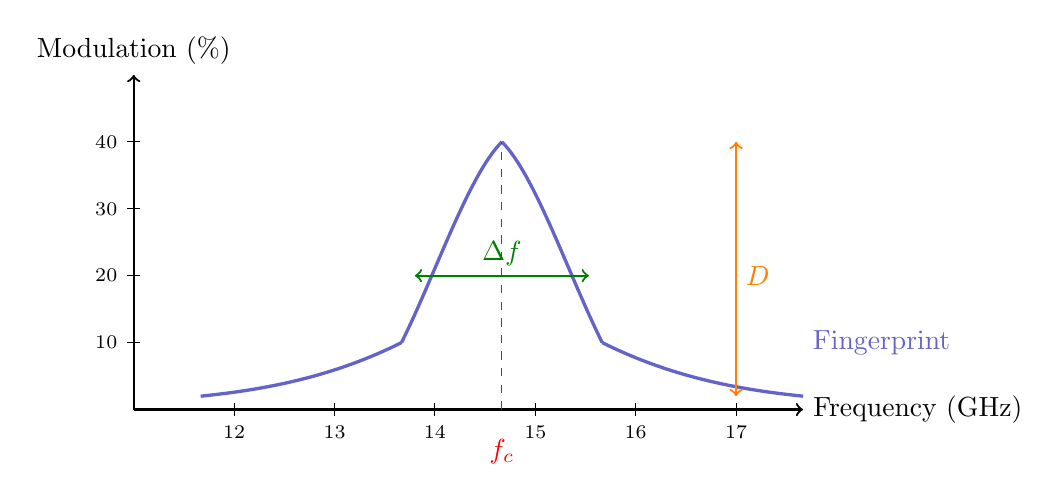
\begin{tikzpicture}[scale=0.85]
    % Axes
    \draw[thick,->] (0,0) -- (10,0) node[right] {Frequency (GHz)};
    \draw[thick,->] (0,0) -- (0,5) node[above] {Modulation (\%)};
    
    % Axis labels
    \foreach \x/\label in {1.5/12, 3/13, 4.5/14, 6/15, 7.5/16, 9/17} {
        \draw (\x,0.1) -- (\x,-0.1) node[below] {\scriptsize \label};
    }
    \foreach \y/\label in {1/10, 2/20, 3/30, 4/40} {
        \draw (0.1,\y) -- (-0.1,\y) node[left] {\scriptsize \label};
    }
    
    % Resonance curve
    \draw[very thick, fingerprint] (1,0.2) .. controls (2,0.3) and (3,0.5) .. (4,1);
    \draw[very thick, fingerprint] (4,1) .. controls (4.5,2) and (5,3.5) .. (5.5,4);
    \draw[very thick, fingerprint] (5.5,4) .. controls (6,3.5) and (6.5,2) .. (7,1);
    \draw[very thick, fingerprint] (7,1) .. controls (8,0.5) and (9,0.3) .. (10,0.2);
    
    % Fingerprint metrics
    \draw[dashed, red] (5.5,0) -- (5.5,4);
    \node[red, below] at (5.5,-0.3) {$f_c$};
    
    \draw[<->, thick, green!50!black] (4.2,2) -- (6.8,2);
    \node[green!50!black, above] at (5.5,2) {$\Delta f$};
    
    \draw[<->, thick, orange] (9,0.2) -- (9,4);
    \node[orange, right] at (9,2) {$D$};
    
    % Labels
    \node[fingerprint, right] at (10,1) {Fingerprint};
    
\end{tikzpicture}
\caption{Resonance fingerprint showing center frequency $f_c$, width $\Delta f$, and depth $D$}
\label{fig:fingerprint}
\end{figure}

\subsection{Objects of the Invention}

It is an object of the present invention to provide methods that:

\begin{enumerate}[label=(\arabic*)]
\item Characterize proteins by their resonance fingerprint;
\item Extract quantitative metrics from resonance curves;
\item Classify proteins and identify variants;
\item Predict aggregation propensity from fingerprint features;
\item Qualify manufacturing lots against reference fingerprints;
\item Verify the resonant mechanism using isotope shift;
\item Provide rapid, non-destructive, label-free assessment.
\end{enumerate}

\newpage

%% ============================================================================
%%                      SUMMARY OF THE INVENTION
%% ============================================================================

\section{SUMMARY OF THE INVENTION}

\subsection{General Statement of the Invention}

The present invention provides methods for protein characterization using resonance fingerprinting, comprising:

\begin{enumerate}[label=(\alph*)]
\item Frequency sweep protocols;
\item Resonance curve fitting;
\item Fingerprint metric extraction;
\item Protein classification and variant identification;
\item Aggregation propensity prediction;
\item Manufacturing lot qualification;
\item Isotope-shift mechanism verification.
\end{enumerate}

\subsection{Fingerprint Metrics}

The fingerprint of a protein is characterized by the following metrics:

\begin{table}[h]
\centering
\begin{tabular}{lll}
\toprule
\textbf{Metric} & \textbf{Symbol} & \textbf{Definition} \\
\midrule
Center frequency & $f_c$ & Frequency of maximum modulation \\
Resonance width & $\Delta f$ & Full width at half maximum (FWHM) \\
Resonance depth & $D$ & Maximum modulation amplitude \\
Asymmetry & $A$ & Skewness of resonance curve \\
Area under curve & $\text{AUC}$ & Integrated modulation \\
Quality factor & $Q$ & $f_c / \Delta f$ \\
\bottomrule
\end{tabular}
\caption{Fingerprint metrics}
\end{table}

\subsection{Application Categories}

\begin{figure}[h]
\centering
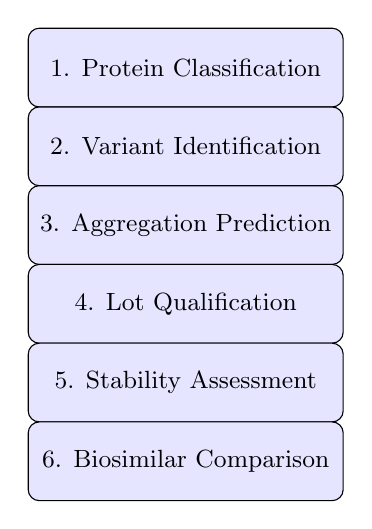
\begin{tikzpicture}[
    app/.style={rectangle, draw, rounded corners, minimum width=4cm, minimum height=1cm, text centered, font=\small, fill=blue!10}
]
    \node[app] at (0,4) {1. Protein Classification};
    \node[app] at (0,3) {2. Variant Identification};
    \node[app] at (0,2) {3. Aggregation Prediction};
    \node[app] at (0,1) {4. Lot Qualification};
    \node[app] at (0,0) {5. Stability Assessment};
    \node[app] at (0,-1) {6. Biosimilar Comparison};
\end{tikzpicture}
\caption{Application categories for resonance fingerprinting}
\label{fig:applications}
\end{figure}

\newpage

%% ============================================================================
%%                    BRIEF DESCRIPTION OF DRAWINGS
%% ============================================================================

\section{BRIEF DESCRIPTION OF DRAWINGS}

\subsection*{Figure 1: Resonance Fingerprint with Metrics}
A graph showing a typical resonance curve with center frequency, width, and depth indicated.

\subsection*{Figure 2: Application Categories}
A list of the six main application categories for resonance fingerprinting.

\subsection*{Figure 3: Frequency Sweep Protocol}
A timing diagram showing the frequency sweep and data acquisition sequence.

\subsection*{Figure 4: Lorentzian Curve Fit}
A graph showing raw data and fitted Lorentzian curve with extracted parameters.

\subsection*{Figure 5: Classification Decision Tree}
A decision tree for classifying proteins based on fingerprint metrics.

\subsection*{Figure 6: Aggregation Risk Score}
A graph showing the correlation between fingerprint metrics and aggregation propensity.

\subsection*{Figure 7: Lot Qualification Workflow}
A flowchart showing the lot qualification process against reference fingerprint.

\subsection*{Figure 8: Isotope Verification Protocol}
A diagram showing the H$_2$O/D$_2$O comparison for mechanism verification.

\newpage

%% ============================================================================
%%                      DETAILED DESCRIPTION
%% ============================================================================

\section{DETAILED DESCRIPTION OF THE PREFERRED EMBODIMENTS}

\subsection{Method 1: Frequency Sweep Protocol}

\subsubsection{Sweep Parameters}

\begin{table}[h]
\centering
\begin{tabular}{lll}
\toprule
\textbf{Parameter} & \textbf{Typical Value} & \textbf{Range} \\
\midrule
Start frequency & 12 GHz & 10--14 GHz \\
Stop frequency & 17 GHz & 15--20 GHz \\
Frequency step & 0.1 GHz & 0.01--0.5 GHz \\
Dwell time per step & 1 s & 0.1--10 s \\
Number of points & 51 & 11--501 \\
Total sweep time & 51 s & 10--500 s \\
Power level & 1 W & 0.1--10 W \\
Sample temperature & 25$^\circ$C & 4--50$^\circ$C \\
\bottomrule
\end{tabular}
\caption{Frequency sweep parameters}
\end{table}

\subsubsection{Sweep Protocol}

\begin{enumerate}[label=(\arabic*)]
\item Prepare protein sample in folding-competent buffer.
\item Equilibrate sample at target temperature.
\item Initiate folding (e.g., denaturant dilution, temperature jump).
\item Begin frequency sweep from $f_{\text{start}}$ to $f_{\text{stop}}$.
\item At each frequency step:
\begin{enumerate}[label=(\alph*)]
\item Set frequency
\item Apply power for dwell time
\item Measure folding response (e.g., fluorescence)
\item Record data point
\end{enumerate}
\item Store complete sweep data for analysis.
\end{enumerate}

\begin{figure}[h]
\centering
\begin{tikzpicture}[scale=0.85]
    % Time axis
    \draw[thick,->] (0,0) -- (12,0) node[right] {Time};
    
    % Frequency steps
    \draw[thick,->] (0,0) -- (0,4) node[above] {Frequency};
    
    % Staircase frequency
    \foreach \x/\y in {0.5/0.5, 1.5/0.8, 2.5/1.1, 3.5/1.4, 4.5/1.7, 5.5/2.0, 6.5/2.3, 7.5/2.6, 8.5/2.9, 9.5/3.2, 10.5/3.5} {
        \draw[thick, blue] (\x,\y) -- (\x+1,\y);
    }
    
    % Data points
    \foreach \x/\y in {1/0.5, 2/0.8, 3/1.1, 4/1.4, 5/1.7, 6/2.0, 7/2.3, 8/2.6, 9/2.9, 10/3.2, 11/3.5} {
        \filldraw[red] (\x,\y) circle (2pt);
    }
    
    % Labels
    \node[blue, right] at (11.5,3.5) {Frequency};
    \node[red, right] at (11.5,2.5) {Data points};
    
    % Dwell time
    \draw[<->, thick] (0.5,-0.5) -- (1.5,-0.5);
    \node[below] at (1,-0.5) {$t_{\text{dwell}}$};
    
\end{tikzpicture}
\caption{Frequency sweep showing stepped frequency and data acquisition}
\label{fig:sweep}
\end{figure}

\subsubsection{Rapid Screening Mode}

For high-throughput applications:
\begin{itemize}
\item Coarse sweep: 0.5 GHz steps, 0.5 s dwell
\item Total time: $\sim$30 s
\item Sufficient for pass/fail determination
\end{itemize}

\subsubsection{High-Resolution Mode}

For detailed characterization:
\begin{itemize}
\item Fine sweep: 0.02 GHz steps, 2 s dwell
\item Total time: $\sim$10 minutes
\item Enables precise metric extraction
\end{itemize}

\subsection{Method 2: Resonance Curve Fitting}

\subsubsection{Lorentzian Model}

The resonance curve is fitted to a Lorentzian function:

\begin{equation}
M(f) = M_0 + \frac{D \cdot (\Delta f / 2)^2}{(f - f_c)^2 + (\Delta f / 2)^2}
\label{eq:lorentz}
\end{equation}

where:
\begin{itemize}
\item $M_0$ = baseline modulation (typically $\sim$0)
\item $D$ = resonance depth (peak height)
\item $f_c$ = center frequency
\item $\Delta f$ = full width at half maximum (FWHM)
\end{itemize}

\subsubsection{Asymmetric Lorentzian Model}

For asymmetric resonances:

\begin{equation}
M(f) = M_0 + \frac{D \cdot (\Delta f / 2)^2}{(f - f_c)^2 + (\Delta f / 2)^2} \times \left[1 + A \cdot \frac{f - f_c}{\Delta f}\right]
\label{eq:asym_lorentz}
\end{equation}

where $A$ is the asymmetry parameter ($A = 0$ for symmetric).

\subsubsection{Gaussian Model (Alternative)}

For broader resonances:

\begin{equation}
M(f) = M_0 + D \cdot \exp\left[-\frac{(f - f_c)^2}{2\sigma^2}\right]
\label{eq:gaussian}
\end{equation}

where $\sigma = \Delta f / (2\sqrt{2\ln 2})$.

\subsubsection{Fitting Algorithm}

\begin{enumerate}[label=(\arabic*)]
\item Initialize parameters from data:
\begin{itemize}
\item $f_c$ = frequency of maximum response
\item $D$ = maximum response value
\item $\Delta f$ = estimated from half-max points
\end{itemize}
\item Perform nonlinear least-squares fit (Levenberg-Marquardt or Trust Region).
\item Calculate goodness-of-fit metrics ($R^2$, $\chi^2$).
\item Extract fitted parameters with confidence intervals.
\end{enumerate}

\begin{figure}[h]
\centering
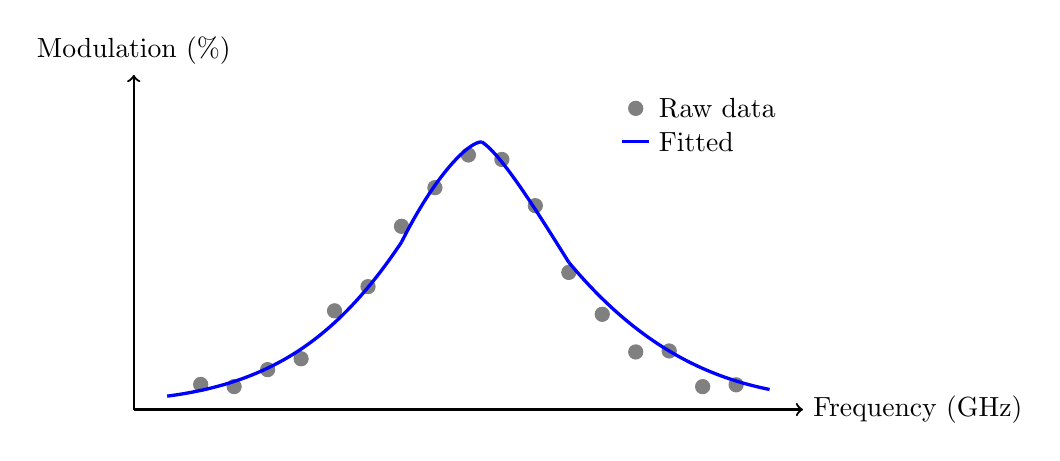
\begin{tikzpicture}[scale=0.85]
    % Axes
    \draw[thick,->] (0,0) -- (10,0) node[right] {Frequency (GHz)};
    \draw[thick,->] (0,0) -- (0,5) node[above] {Modulation (\%)};
    
    % Raw data points (noisy)
    \foreach \x/\y in {1/0.3, 1.5/0.4, 2/0.6, 2.5/0.9, 3/1.3, 3.5/2.0, 4/2.8, 4.5/3.5, 5/4.0, 5.5/3.6, 6/2.9, 6.5/2.1, 7/1.4, 7.5/1.0, 8/0.7, 8.5/0.5, 9/0.4} {
        \filldraw[gray] (\x,\y+0.2*rand) circle (3pt);
    }
    
    % Fitted curve
    \draw[very thick, blue] (0.5,0.2) .. controls (2,0.4) and (3,1) .. (4,2.5);
    \draw[very thick, blue] (4,2.5) .. controls (4.5,3.5) and (5,4) .. (5.2,4);
    \draw[very thick, blue] (5.2,4) .. controls (5.5,3.8) and (6,3) .. (6.5,2.2);
    \draw[very thick, blue] (6.5,2.2) .. controls (7.5,1) and (8.5,0.5) .. (9.5,0.3);
    
    % Legend
    \filldraw[gray] (7.5,4.5) circle (3pt);
    \node[right] at (7.7,4.5) {Raw data};
    \draw[very thick, blue] (7.3,4) -- (7.7,4);
    \node[right] at (7.7,4) {Fitted};
    
\end{tikzpicture}
\caption{Lorentzian fit to raw frequency sweep data}
\label{fig:fit}
\end{figure}

\subsection{Method 3: Fingerprint Metric Extraction}

\subsubsection{Primary Metrics}

From the fitted curve:

\begin{table}[h]
\centering
\begin{tabular}{llll}
\toprule
\textbf{Metric} & \textbf{Formula} & \textbf{Typical Value} & \textbf{Units} \\
\midrule
Center frequency & $f_c$ & 14.65 & GHz \\
Width (FWHM) & $\Delta f$ & 0.5--2.0 & GHz \\
Depth & $D$ & 30--50 & \% \\
Quality factor & $Q = f_c / \Delta f$ & 7--30 & dimensionless \\
Asymmetry & $A$ & $-0.5$ to $+0.5$ & dimensionless \\
\bottomrule
\end{tabular}
\caption{Primary fingerprint metrics}
\end{table}

\subsubsection{Derived Metrics}

\begin{enumerate}[label=(\arabic*)]
\item \textbf{Area under curve (AUC):}
\begin{equation}
\text{AUC} = \int_{f_{\text{start}}}^{f_{\text{stop}}} M(f) \, df \approx \frac{\pi D \Delta f}{2}
\label{eq:auc}
\end{equation}

\item \textbf{Frequency shift from reference:}
\begin{equation}
\delta f = f_c - f_{\text{ref}}
\label{eq:shift}
\end{equation}

\item \textbf{Width ratio:}
\begin{equation}
W_{\text{ratio}} = \frac{\Delta f}{\Delta f_{\text{ref}}}
\label{eq:wratio}
\end{equation}

\item \textbf{Depth ratio:}
\begin{equation}
D_{\text{ratio}} = \frac{D}{D_{\text{ref}}}
\label{eq:dratio}
\end{equation}
\end{enumerate}

\subsubsection{Fingerprint Vector}

The complete fingerprint is represented as a vector:

\begin{equation}
\mathbf{F} = [f_c, \Delta f, D, A, Q, \text{AUC}]^T
\label{eq:vector}
\end{equation}

This vector enables quantitative comparison between samples.

\subsection{Method 4: Protein Classification}

\subsubsection{Classification by Fingerprint Similarity}

Proteins are classified by comparing their fingerprint vector $\mathbf{F}$ to reference fingerprints $\mathbf{F}_i$ for known protein classes:

\begin{equation}
\text{Distance}_i = \|\mathbf{F} - \mathbf{F}_i\|_W = \sqrt{\sum_j w_j (F_j - F_{i,j})^2}
\label{eq:distance}
\end{equation}

where $w_j$ are metric weights.

The protein is assigned to the class with minimum distance:

\begin{equation}
\text{Class} = \arg\min_i \text{Distance}_i
\label{eq:class}
\end{equation}

\subsubsection{Classification Features}

\begin{table}[h]
\centering
\begin{tabular}{lll}
\toprule
\textbf{Feature} & \textbf{Distinguishes} & \textbf{Mechanism} \\
\midrule
Center frequency & Protein identity & Gate timescale \\
Width & Folding cooperativity & Transition state barrier \\
Depth & Folding efficiency & Resonant coupling strength \\
Asymmetry & Structural heterogeneity & Multiple populations \\
Quality factor & Folding pathway complexity & Gate sharpness \\
\bottomrule
\end{tabular}
\caption{Classification features and their physical meaning}
\end{table}

\subsubsection{Decision Tree Classification}

\begin{figure}[h]
\centering
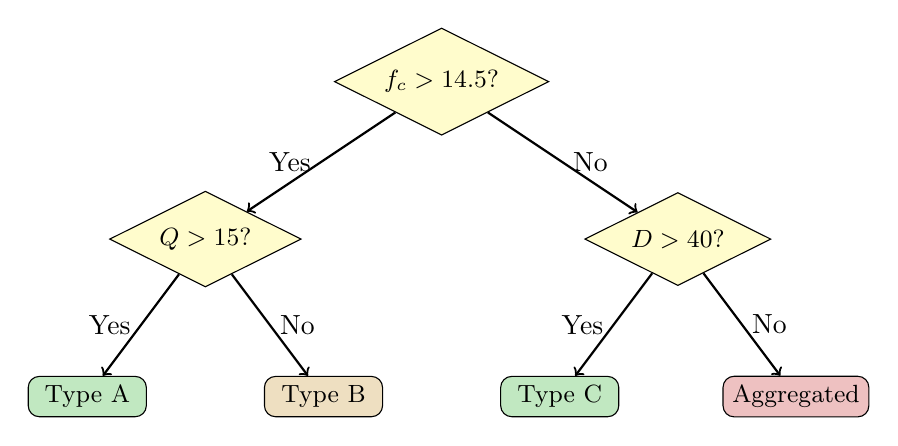
\begin{tikzpicture}[
    decision/.style={diamond, draw, minimum width=2cm, text centered, font=\small, aspect=2},
    result/.style={rectangle, draw, rounded corners, minimum width=1.5cm, text centered, font=\small},
    arrow/.style={->, thick}
]
    % Root
    \node[decision, fill=yellow!20] (root) at (5,6) {$f_c > 14.5$?};
    
    % Level 1
    \node[decision, fill=yellow!20] (l1a) at (2,4) {$Q > 15$?};
    \node[decision, fill=yellow!20] (l1b) at (8,4) {$D > 40$?};
    
    % Results
    \node[result, fill=pass!30] (r1) at (0.5,2) {Type A};
    \node[result, fill=warning!30] (r2) at (3.5,2) {Type B};
    \node[result, fill=pass!30] (r3) at (6.5,2) {Type C};
    \node[result, fill=fail!30] (r4) at (9.5,2) {Aggregated};
    
    % Arrows
    \draw[arrow] (root) -- node[left] {Yes} (l1a);
    \draw[arrow] (root) -- node[right] {No} (l1b);
    \draw[arrow] (l1a) -- node[left] {Yes} (r1);
    \draw[arrow] (l1a) -- node[right] {No} (r2);
    \draw[arrow] (l1b) -- node[left] {Yes} (r3);
    \draw[arrow] (l1b) -- node[right] {No} (r4);
    
\end{tikzpicture}
\caption{Example decision tree for protein classification}
\label{fig:tree}
\end{figure}

\subsection{Method 5: Aggregation Propensity Prediction}

\subsubsection{Aggregation Markers}

Certain fingerprint features correlate with aggregation propensity:

\begin{table}[h]
\centering
\begin{tabular}{lll}
\toprule
\textbf{Feature} & \textbf{Aggregation-Prone} & \textbf{Aggregation-Resistant} \\
\midrule
Width $\Delta f$ & Broad ($>$ 1.5 GHz) & Narrow ($<$ 1.0 GHz) \\
Quality factor $Q$ & Low ($<$ 10) & High ($>$ 20) \\
Asymmetry $|A|$ & Large ($>$ 0.3) & Small ($<$ 0.1) \\
Multiple peaks & Present & Absent \\
\bottomrule
\end{tabular}
\caption{Fingerprint features correlated with aggregation propensity}
\end{table}

\subsubsection{Aggregation Risk Score}

An aggregation risk score is computed as a weighted combination:

\begin{equation}
\text{Risk} = w_1 \cdot \frac{\Delta f}{\Delta f_{\text{ref}}} + w_2 \cdot \frac{Q_{\text{ref}}}{Q} + w_3 \cdot |A| + w_4 \cdot N_{\text{peaks}}
\label{eq:risk}
\end{equation}

where $N_{\text{peaks}}$ is the number of resolved peaks.

\subsubsection{Risk Categories}

\begin{table}[h]
\centering
\begin{tabular}{lll}
\toprule
\textbf{Risk Score} & \textbf{Category} & \textbf{Action} \\
\midrule
$<$ 1.0 & Low risk & Normal processing \\
1.0--2.0 & Moderate risk & Enhanced monitoring \\
2.0--3.0 & High risk & Formulation optimization \\
$>$ 3.0 & Very high risk & Reject or re-engineer \\
\bottomrule
\end{tabular}
\caption{Aggregation risk categories}
\end{table}

\subsection{Method 6: Manufacturing Lot Qualification}

\subsubsection{Reference Fingerprint Establishment}

For a new protein product:
\begin{enumerate}[label=(\arabic*)]
\item Characterize multiple ($\geq$ 10) reference lots known to meet specifications.
\item Compute mean fingerprint vector $\bar{\mathbf{F}}$ and covariance matrix $\mathbf{\Sigma}$.
\item Define acceptance limits based on statistical analysis.
\end{enumerate}

\subsubsection{Lot Testing Protocol}

For each production lot:
\begin{enumerate}[label=(\arabic*)]
\item Perform frequency sweep on representative sample.
\item Fit resonance curve and extract fingerprint $\mathbf{F}_{\text{lot}}$.
\item Compute Mahalanobis distance from reference:
\begin{equation}
d_M = \sqrt{(\mathbf{F}_{\text{lot}} - \bar{\mathbf{F}})^T \mathbf{\Sigma}^{-1} (\mathbf{F}_{\text{lot}} - \bar{\mathbf{F}})}
\label{eq:mahal}
\end{equation}
\item Compare to acceptance threshold.
\end{enumerate}

\subsubsection{Acceptance Criteria}

\begin{table}[h]
\centering
\begin{tabular}{lll}
\toprule
\textbf{Distance $d_M$} & \textbf{Result} & \textbf{Confidence} \\
\midrule
$<$ 2.0 & Pass & $>$ 95\% \\
2.0--3.0 & Conditional & Investigate \\
$>$ 3.0 & Fail & $<$ 95\% \\
\bottomrule
\end{tabular}
\caption{Lot acceptance criteria based on Mahalanobis distance}
\end{table}

\begin{figure}[h]
\centering
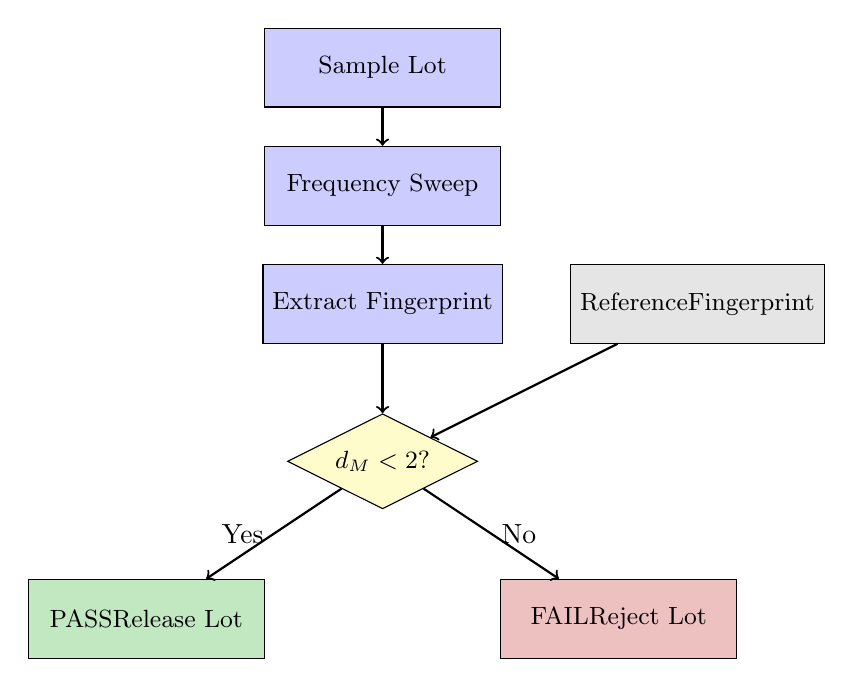
\begin{tikzpicture}[
    block/.style={rectangle, draw, minimum width=3cm, minimum height=1cm, text centered, font=\small},
    decision/.style={diamond, draw, minimum width=2cm, text centered, font=\small, aspect=2},
    arrow/.style={->, thick}
]
    % Blocks
    \node[block, fill=blue!20] (sample) at (0,5) {Sample Lot};
    \node[block, fill=blue!20] (sweep) at (0,3.5) {Frequency Sweep};
    \node[block, fill=blue!20] (extract) at (0,2) {Extract Fingerprint};
    \node[decision, fill=yellow!20] (compare) at (0,0) {$d_M < 2$?};
    \node[block, fill=pass!30] (pass) at (-3,-2) {PASS\\Release Lot};
    \node[block, fill=fail!30] (fail) at (3,-2) {FAIL\\Reject Lot};
    
    % Reference
    \node[block, fill=gray!20] (ref) at (4,2) {Reference\\Fingerprint};
    
    % Arrows
    \draw[arrow] (sample) -- (sweep);
    \draw[arrow] (sweep) -- (extract);
    \draw[arrow] (extract) -- (compare);
    \draw[arrow] (ref) -- (compare);
    \draw[arrow] (compare) -- node[left] {Yes} (pass);
    \draw[arrow] (compare) -- node[right] {No} (fail);
    
\end{tikzpicture}
\caption{Lot qualification workflow}
\label{fig:lot_qual}
\end{figure}

\subsection{Method 7: Isotope-Shift Verification}

\subsubsection{Verification Protocol}

To confirm that the fingerprint reflects a resonant mechanism (not thermal artifact):

\begin{enumerate}[label=(\arabic*)]
\item Perform H$_2$O frequency sweep; extract $f_c^{\text{H}_2\text{O}}$.
\item Prepare equivalent sample in D$_2$O.
\item Perform D$_2$O frequency sweep (8--13 GHz); extract $f_c^{\text{D}_2\text{O}}$.
\item Verify isotope ratio:
\begin{equation}
R = \frac{f_c^{\text{H}_2\text{O}}}{f_c^{\text{D}_2\text{O}}} = \sqrt{2} \pm 5\%
\label{eq:ratio}
\end{equation}
\end{enumerate}

\subsubsection{Verification Criteria}

\begin{table}[h]
\centering
\begin{tabular}{lll}
\toprule
\textbf{Ratio $R$} & \textbf{Conclusion} & \textbf{Action} \\
\midrule
1.35--1.49 & Resonant confirmed & Use fingerprint \\
1.05--1.25 & Thermal mechanism & Investigate \\
Other & Invalid data & Repeat measurement \\
\bottomrule
\end{tabular}
\caption{Isotope verification criteria}
\end{table}

\subsubsection{Combined Fingerprint}

A verified fingerprint includes both H$_2$O and D$_2$O measurements:

\begin{equation}
\mathbf{F}_{\text{verified}} = [\mathbf{F}^{\text{H}_2\text{O}}, \mathbf{F}^{\text{D}_2\text{O}}, R]^T
\label{eq:verified}
\end{equation}

This extended fingerprint provides additional discriminating power.

\subsection{Application Examples}

\subsubsection{Biosimilar Comparison}

Compare biosimilar to innovator product:
\begin{enumerate}[label=(\arabic*)]
\item Establish innovator fingerprint from multiple lots.
\item Measure biosimilar fingerprint.
\item Compute similarity score:
\begin{equation}
S = 1 - \frac{d_M}{d_{\text{max}}}
\label{eq:similarity}
\end{equation}
\item Report similarity percentage.
\end{enumerate}

\subsubsection{Stability Assessment}

Monitor stability over time:
\begin{enumerate}[label=(\arabic*)]
\item Establish $t = 0$ fingerprint.
\item Store samples under various conditions.
\item Measure fingerprints at time points.
\item Track fingerprint drift vs.\ time.
\item Predict shelf life from drift rate.
\end{enumerate}

\subsubsection{Process Development}

Optimize manufacturing process:
\begin{enumerate}[label=(\arabic*)]
\item Vary process parameters (pH, temperature, mixing, etc.).
\item Measure fingerprint at each condition.
\item Identify parameters that maximize $Q$ and minimize $\Delta f$.
\item Select optimal conditions.
\end{enumerate}

\subsection{Performance Specifications}

\begin{table}[h]
\centering
\begin{tabular}{lll}
\toprule
\textbf{Metric} & \textbf{Specification} & \textbf{Notes} \\
\midrule
Measurement time & $<$ 10 minutes & Standard mode \\
Rapid screening & $<$ 1 minute & Reduced resolution \\
Frequency accuracy & $\pm$0.05 GHz & Center frequency \\
Width accuracy & $\pm$0.1 GHz & FWHM \\
Depth accuracy & $\pm$5\% & Relative \\
Repeatability & CV $<$ 5\% & Same sample \\
Sample volume & 50--500 $\mu$L & Standard cuvette \\
Protein concentration & 0.1--10 mg/mL & Working range \\
\bottomrule
\end{tabular}
\caption{Performance specifications for resonance fingerprinting}
\end{table}

\newpage

%% ============================================================================
%%                              CLAIMS
%% ============================================================================

\section{CLAIMS}

What is claimed is:

\subsection{Frequency Sweep Claims}

\begin{enumerate}[label=\textbf{\arabic*.}]

\item A method for characterizing a protein using resonance fingerprinting, comprising:
\begin{enumerate}[label=(\alph*)]
\item preparing a sample of the protein in an aqueous buffer;
\item performing a frequency sweep by irradiating the sample with electromagnetic radiation at a plurality of frequencies in the range of 12 to 17 GHz;
\item measuring a folding response at each frequency;
\item recording the folding response as a function of frequency to obtain a resonance curve; and
\item extracting one or more fingerprint metrics from the resonance curve.
\end{enumerate}

\item The method of claim 1, wherein the fingerprint metrics include one or more of: center frequency, resonance width (FWHM), resonance depth, asymmetry, area under curve, and quality factor.

\item The method of claim 1, wherein the frequency sweep comprises at least 20 frequency points with a frequency step of 0.5 GHz or less.

\item The method of claim 1, wherein the total measurement time is less than 10 minutes.

\end{enumerate}

\subsection{Curve Fitting Claims}

\begin{enumerate}[label=\textbf{\arabic*.}]
\setcounter{enumi}{4}

\item A method for extracting fingerprint metrics from a resonance curve, comprising:
\begin{enumerate}[label=(\alph*)]
\item fitting the resonance curve to a model function selected from Lorentzian, asymmetric Lorentzian, and Gaussian;
\item extracting fitted parameters including center frequency $f_c$, width $\Delta f$, and depth $D$;
\item computing derived metrics including quality factor $Q = f_c / \Delta f$ and area under curve; and
\item storing the extracted metrics as a fingerprint vector.
\end{enumerate}

\item The method of claim 5, wherein the fitting is performed using nonlinear least-squares optimization.

\item The method of claim 5, further comprising computing confidence intervals for the extracted parameters.

\end{enumerate}

\subsection{Classification Claims}

\begin{enumerate}[label=\textbf{\arabic*.}]
\setcounter{enumi}{7}

\item A method for classifying a protein based on its resonance fingerprint, comprising:
\begin{enumerate}[label=(\alph*)]
\item obtaining a fingerprint vector for the protein according to claims 1--5;
\item comparing the fingerprint vector to a database of reference fingerprints for known protein classes;
\item computing a distance or similarity measure between the fingerprint and each reference; and
\item assigning the protein to the class with the smallest distance or highest similarity.
\end{enumerate}

\item The method of claim 8, wherein the distance measure is Euclidean distance with optional weighting.

\item The method of claim 8, wherein the distance measure is Mahalanobis distance accounting for covariance structure.

\item The method of claim 8, wherein classification is performed using a decision tree, random forest, or neural network trained on reference fingerprints.

\end{enumerate}

\subsection{Aggregation Prediction Claims}

\begin{enumerate}[label=\textbf{\arabic*.}]
\setcounter{enumi}{11}

\item A method for predicting aggregation propensity of a protein, comprising:
\begin{enumerate}[label=(\alph*)]
\item obtaining a fingerprint for the protein according to claims 1--5;
\item computing an aggregation risk score based on fingerprint metrics;
\item classifying the protein into a risk category based on the score; and
\item outputting the risk category and/or a recommendation for handling.
\end{enumerate}

\item The method of claim 12, wherein the aggregation risk score is computed from one or more of: resonance width, quality factor, asymmetry, and number of resolved peaks.

\item The method of claim 12, wherein a broader resonance width indicates higher aggregation propensity.

\item The method of claim 12, wherein the presence of multiple peaks indicates structural heterogeneity and elevated aggregation risk.

\end{enumerate}

\subsection{Lot Qualification Claims}

\begin{enumerate}[label=\textbf{\arabic*.}]
\setcounter{enumi}{15}

\item A method for qualifying a manufacturing lot of a protein product, comprising:
\begin{enumerate}[label=(\alph*)]
\item establishing a reference fingerprint from multiple qualified reference lots;
\item obtaining a fingerprint for a sample from the manufacturing lot to be qualified;
\item computing a distance between the lot fingerprint and the reference fingerprint;
\item comparing the distance to an acceptance threshold; and
\item generating a pass or fail determination based on the comparison.
\end{enumerate}

\item The method of claim 16, wherein the reference fingerprint comprises a mean fingerprint vector and a covariance matrix.

\item The method of claim 16, wherein the distance is Mahalanobis distance and the acceptance threshold corresponds to a 95\% confidence region.

\item The method of claim 16, further comprising storing the lot fingerprint and qualification result in a database for trending analysis.

\end{enumerate}

\subsection{Isotope Verification Claims}

\begin{enumerate}[label=\textbf{\arabic*.}]
\setcounter{enumi}{19}

\item A method for verifying that a resonance fingerprint reflects a resonant mechanism, comprising:
\begin{enumerate}[label=(\alph*)]
\item obtaining a fingerprint in H$_2$O with center frequency $f_c^{\text{H}_2\text{O}}$;
\item obtaining a fingerprint in D$_2$O with center frequency $f_c^{\text{D}_2\text{O}}$;
\item computing the frequency ratio $R = f_c^{\text{H}_2\text{O}} / f_c^{\text{D}_2\text{O}}$; and
\item confirming a resonant mechanism if $R = \sqrt{2}$ within a tolerance of $\pm$5\%.
\end{enumerate}

\item The method of claim 20, wherein the D$_2$O fingerprint is obtained by performing a frequency sweep in the range of 8 to 13 GHz.

\item The method of claim 20, further comprising generating a verified fingerprint that includes both H$_2$O and D$_2$O metrics and the frequency ratio.

\end{enumerate}

\subsection{System Claims}

\begin{enumerate}[label=\textbf{\arabic*.}]
\setcounter{enumi}{22}

\item A system for protein resonance fingerprinting, comprising:
\begin{enumerate}[label=(\alph*)]
\item a frequency-tunable microwave source;
\item a sample chamber configured to hold a protein sample;
\item a folding detector configured to measure protein folding response;
\item a processor configured to control the frequency sweep, record data, fit the resonance curve, and extract fingerprint metrics; and
\item a database configured to store reference fingerprints and test results.
\end{enumerate}

\item The system of claim 23, further comprising a report generator configured to output pass/fail determinations, similarity scores, and risk assessments.

\item A non-transitory computer-readable medium storing instructions that, when executed by a processor, cause the processor to perform the method of any of claims 1--22.

\end{enumerate}

\newpage

%% ============================================================================
%%                         ABSTRACT
%% ============================================================================

\section*{ABSTRACT}
\addcontentsline{toc}{section}{ABSTRACT}

Methods for characterizing proteins using resonance fingerprinting based on the molecular gate frequency. The methods comprise: (1) performing a frequency sweep across 12--17 GHz (H$_2$O) or 8--13 GHz (D$_2$O) while monitoring protein folding response; (2) fitting the resonance curve to a Lorentzian or related model to extract fingerprint metrics including center frequency, width (FWHM), depth, asymmetry, area under curve, and quality factor; (3) representing the fingerprint as a vector for quantitative comparison; (4) classifying proteins by comparing fingerprints to reference databases using distance metrics or machine learning; (5) predicting aggregation propensity from fingerprint features (broad width, low quality factor, multiple peaks); (6) qualifying manufacturing lots by computing Mahalanobis distance from reference fingerprint with statistical acceptance criteria; and (7) verifying the resonant mechanism by confirming a $\sqrt{2}$ isotope shift between H$_2$O and D$_2$O measurements. The methods enable rapid ($<$ 10 minutes), non-destructive, label-free characterization of protein folding dynamics with applications in biopharmaceutical manufacturing quality control, lot release testing, biosimilar comparison, stability assessment, and research protein characterization. Performance specifications include frequency accuracy of $\pm$0.05 GHz, repeatability CV $<$ 5\%, and working protein concentration range of 0.1--10 mg/mL.

\vspace{1in}

\begin{center}
\textbf{--- END OF SPECIFICATION ---}
\end{center}

\newpage

%% ============================================================================
%%                         INVENTOR DECLARATION
%% ============================================================================

\section*{INVENTOR DECLARATION}
\addcontentsline{toc}{section}{INVENTOR DECLARATION}

I, Jonathan Washburn, declare that:

\begin{enumerate}[label=(\arabic*)]
\item I am the original and sole inventor of the resonance fingerprinting methods described and claimed in this application.

\item I have reviewed the above specification and claims and believe them to be accurate and complete.

\item I believe the claimed invention to be novel, useful, and non-obvious over the prior art.

\item I authorize the filing of this provisional patent application to establish a priority date.
\end{enumerate}

\vspace{1in}

\noindent\textbf{Inventor Signature:} \hrulefill

\vspace{0.5in}

\noindent\textbf{Name:} Jonathan Washburn

\noindent\textbf{Email:} washburn.jonathan@gmail.com

\noindent\textbf{Date:} \hrulefill

\vspace{1in}

\begin{center}
\textit{This document is intended for provisional patent application filing purposes.\\
All information contained herein is confidential and proprietary.}
\end{center}

\end{document}
